\section{Materials}
This setup for measuring energy consumption includes an Arduino microcontroller and a Current Transformer (CT) sensor. The CT sensor detects the alternating current (AC) flowing through a conductor without direct electrical contact. It outputs a proportional current signal to the Arduino, which processes the data to calculate energy consumption. To improve accuracy, the system may include resistors, capacitors for filtering, and a voltage divider circuit for safe scaling, allowing the Arduino to measure and record energy data reliably for applications like household or small industrial monitoring.

\subsection{Arduino Microcontroller UNO}
\begin{figure}[H]
    \centering
    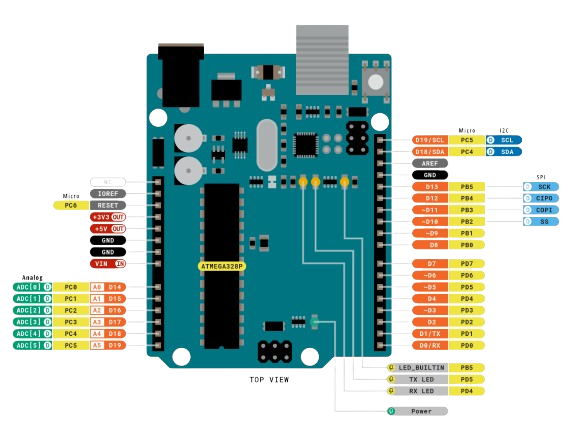
\includegraphics[width=\linewidth]{Graphics/ard_uno-removebg-preview.png}
    \caption{Arduino Uno Microcontroller}
    \label{fig:image1}
\end{figure}
The Arduino UNO is the core microcontroller for this energy monitoring setup, handling data from various sensors and executing calculations for accurate energy measurements. It operates on a 5V logic level, suitable for reading data from components like the CT sensor (current transformer) and voltage divider circuits. Potential additional components include resistors to limit current, capacitors to filter noise, and an external analog-to-digital converter if higher accuracy is needed. \cite{OpenEnergyMonitor_Arduino}

\subsection{YHDC Current Transformer SCT-013-000}
\begin{minipage}{\linewidth}
\begin{figure}[H]
\centering
    \begin{circuitikz}
        \tikzstyle{every node}=[font=\small]
        \draw [](1.25,11.5) to[short] (3,11.5);
        \draw [](1.25,11.5) to[short, -o] (0.75,11.5);
        \draw [->, >=Stealth] (1.75,11.5) -- (2,11.5);
        
        \draw [](3,11.5) to[short] (3,10.75);
        \draw [](3,11) to[short] (3,10.5);
        \draw (3,10.5) to[L ] (5,10.5);
        
        \draw [](5,10.5) to[short] (5,11.5);
        \draw [](5,11.5) to[short] (6.5,11.5);
        \draw [](6.5,11.5) to[short, -o] (7,11.5) ;
        \draw [->, >=Stealth] (6,11.5) -- (6.25,11.5);
        \draw (2.75,9.5) to[L ] (5.25,9.5);
        
        \draw[] (5.25,9.5) to[short] (5,9.5);
        
        \draw[] (5,9.5) to[short] (4.75,9.5);
        \draw [, dashed] (2.75,11) rectangle  (5.25,9.25);
        \draw [](2.75,9.25) to[short] (2.75,8.75);
        \draw [](2.75,8.75) to[short] (2.75,8.25);
        
        \draw [](5.25,9.25) to[short] (5.25,8.25);
        \draw[] (5.25,8.25) to[short] (4.5,8.25);
        \node at (4.5,8.25) [circ] {};
        \draw [](4.5,8.25) to[short] (4.5,6.25);
        \node at (2.75,8.25) [circ] {};
        
        \draw [](2.75,8.25) to[short] (2.75,5.75);
        \draw (2.25,7.25) to[C] (1.5,7.25);
        \node at (2.75,7.25) [circ] {};
        \draw (2.25,7.25) to[C] (1,7.25);
        \draw [](2.75,5.75) to[short] (2.75,5.5);
        \draw [](2.75,5.5) to[short] (2.75,5.25);
        \node at (2.75,5.25) [circ] {};
        \draw (2.75,5.25) to[R] (4.75,5.25);
        \draw (2.25,5.25) to[R] (1,5.25);
        \draw [](2.25,5.25) to[short] (2.75,5.25);
        \draw [](2.25,7.25) to[short] (2.75,7.25);
        \draw[] (1,5.25) to[short] (0.75,5.25);
        \draw[] (1,7.25) to[short] (0.75,7.25);
        \draw[] (0.75,5.25) to[short] (0.5,5.25);
        \draw[] (0.75,7.25) to[short] (0.5,7.25);
        \node at (0.5,7.25) [circ] {};
        \node at (0.5,5.25) [circ] {};
        \draw [](0.5,5.25) to[short] (0.5,7.25);
        \draw [](0.5,7.25) to[short] (0.5,8.25);
        \draw [](0.5,5.25) to[short] (0.5,4);
        \draw [](2.75,5.25) to[short] (2.75,4.25);
        \draw [](2.75,4.25) to[short] (2.75,4);
        \draw [](4.5,6.25) to[short] (4.5,4);
        \draw [](4.5,5.25) to[short] (5,5.25);
        \draw [](4.75,5.25) to[short] (5.5,5.25);
        \draw [](5.5,5.25) to[short] (5.5,4);
        \node [font=\small] at (1.75,11.75) {Heavy line current};
        \node [font=\small] at (6.75,10) {Current transformer};
        \node [font=\small] at (4,9) {Secondary};
        \node [font=\small] at (4,11.25) {Primary};
        \node [font=\small] at (6,11.75) {To load};
        \node [font=\small] at (1.75,8) {C1 10$\mu$F};
        \node [font=\small] at (1.75,5.75) {R1 10k$\Omega$};
        \node [font=\small] at (3.75,5.75) {R2 10k$\Omega$};
        \draw [](2.75,8.25) to[short] (4.5,8.25);
        \node [font=\small] at (6.25,8.75) {C.T Output};
        \node [font=\small, rotate around={270:(0,0)}] at (0.25,4.5) {Arduino GND};
        \node [font=\small, rotate around={270:(0,0)}] at (4.25,4) {Arduino input};
        \node [font=\small, rotate around={270:(0,0)}] at (5.75,4.5) {Arduino 5V DC};
        \node [font=\small, rotate around={270:(0,0)}] at (2.5,4.5) {Mid-point};
        \draw [](5.5,3.75) to[short, o-] (5.5,4) ;
        \draw [](0.5,3.75) to[short, o-] (0.5,4) ;
        \draw [](4.5,3.75) to[short, o-] (4.5,4) ;
        \draw [](2.75,4) to[short] (2.75,3.75);
    \end{circuitikz}
    \caption{Current transformer circuit with Arduino}
    \label{fig:CT - Sensor}
\end{figure}
\vspace{2pt}
\end{minipage}
The YHDC SCT-013-000 is a non-invasive current transformer sensor used to measure AC current without direct contact with the high-voltage line. This CT sensor detects current based on electromagnetic induction and outputs a small, proportional AC signal. When connected to the Arduino, it allows accurate monitoring of the current flowing through the conductor. With the help of filtering capacitors and resistors for scaling, the output signal from the CT sensor is adapted to the Arduino’s input range, enabling precise energy calculations. \cite{OpenEnergyMonitor_Arduino}

\subsection{Liquid Crystal Display}
\begin{itemize}
    \item Display: It displays information like voltage, current, power consumption, and other relevant data. \cite{techtarget_lcd}
    \item Backlight: It provides illumination for better visibility. \cite{techtarget_lcd}
    \item Interface: It connects to the Arduino board through digital pins to receive and display data.
    \item Types: There are various types of LCDs, including character LCDs and graphic LCDs.
\end{itemize}

\subsection{ Potential Components:}
\begin{itemize}
    \item Voltage Sensor: To measure voltage, we initially tried the Open Energy Monitor (EmonLib) approach, which utilizes an AC-AC adapter to capture the alternating voltage signal. However, due to issues with stability, we instead used a fixed AC voltage source of 127V for this setup. This consistent voltage ensures a reliable reference for calculating power and energy consumption.
    \item Temperature Sensor: Monitors the temperature of the system or environment.
    \item Power Supply: Provides the necessary power for the Arduino and other components.
    \item LCD (Liquid Crystal Display):
\end{itemize}

\subsection{Voltage Divider}
The voltage divider circuit is designed to scale down the high input voltage of 127V AC to a safe range of 0-5V DC for Arduino's analog input. It consists of two resistors ($R_1$ and $R_2$) that divide the voltage proportionally based on their resistance values. A capacitor ($C_1$) is added to filter noise, and a coupling capacitor ($C_2$) biases the signal within the 0-5V range. This enables the Arduino to read the AC signal safely without risking damage from high voltage. \cite{OpenEnergyMonitor_Voltage}

The output voltage, $V_{out}$, can be calculated as:
$$ V_{out} = V_{in} \times \frac{R_2}{R_1 + R_2}$$

where $V_{in}$ is the input AC voltage (127V). By selecting appropriate resistor values, $V_{out}$ can be scaled to fall within the Arduino's input limits.
��\begin{figure}[H]

    \begin{minipage}{\linewidth}

        \begin{center}

            \begin{circuitikz}[scale=0.8, transform shape] % Scale and avoid shape deformation

                % AC-AC Adapter

                \draw (0,4) node[vsource, rotate=-90] (AC) {}

                    (AC.north) node[above=0.3cm] {$\sim$ AC-AC Adapter};



                % First Resistor (R1) in Voltage Divider

                \draw (AC.south)

                      to[R=$R_1$, *-*] (0,2) coordinate (R1R2);



                % Second Resistor (R2) in Voltage Divider

                \draw (R1R2) to[R=$R_2$, *-*] (0,0) coordinate (ground);



                % Capacitor (C1) to Filter Signal

                \draw (R1R2) -- (2,2)

                      to[C=$C_1$] (2,0) -- (ground);



                % Reference Voltage Bias with Resistors (R3 and R4)

                \draw (3,4) to[R=$R_3$] (3,2) coordinate (bias)

                            to[R=$R_4$] (3,0);

                \draw (3,0) node[ground] {};



                % Connect Bias Point to Voltage Divider Output via Coupling Capacitor (C2)

                \draw (R1R2) -- (1,2) to[C=$C_2$] (1.5,2) -- (bias);



                % Arduino Analog Input

                \draw (bias) -- (5,2) node[right, xshift=0.3cm] {Arduino Analog Pin};



                % Labels

                \node at (1,3.5) {$V_{in}$}; % Adjusted label position

                \node at (4.5,2.5) {$V_{out}$ (0-5V range)}; % Adjusted label position

                \node at (1.6,0.5) {Ground}; % Adjusted label position



            \end{circuitikz}

        \end{center}

        \caption{Voltage Divider with Filtering and Biasing for Arduino Analog Input}

        \label{fig:voltage-divider}

    \end{minipage}

    \end{figure}


The circuit is designed to measure AC voltage using an Arduino, an AC-AC power adapter, and a voltage divider. The AC-AC adapter supplies the input voltage (\(V_{\text{in}}\)) to the circuit. The voltage divider, made of resistors \(R_1\) and \(R_2\), steps down the AC voltage to a safe level for the Arduino’s 0-5V input range. The resistors are selected to ensure the voltage stays within the Arduino’s limits.

To allow the Arduino to read both positive and negative portions of the AC waveform, the signal is biased to a 2.5V reference using resistors \(R_3\) and \(R_4\). Capacitor \(C_1\) filters high-frequency noise, ensuring clean signal measurement. A coupling capacitor (\(C_2\)) isolates the DC bias while passing the AC signal to the Arduino’s analog input, where it is digitized for further analysis. This setup enables safe, accurate measurement of AC voltage for energy monitoring. \cite{OpenEnergyMonitor_Voltage}
\begin{minipage}{\linewidth}  % Minipage with full line width
    \vspace{1cm}
        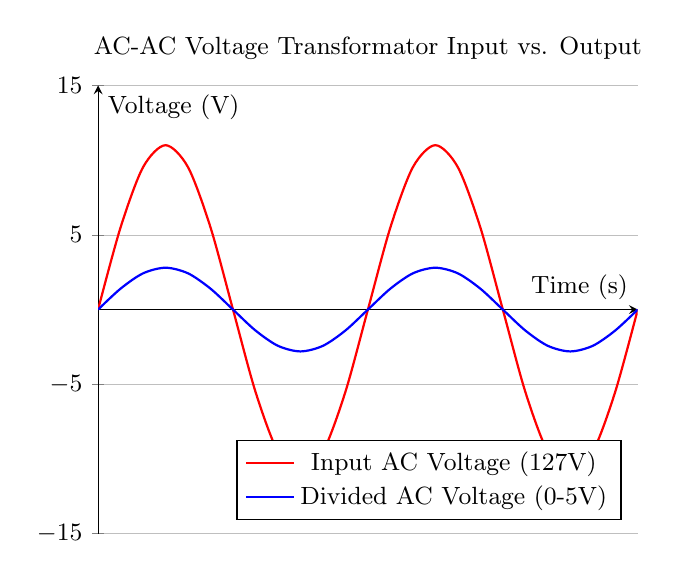
\begin{tikzpicture}
            \begin{axis}[
                title={AC-AC Voltage Transformator Input vs. Output},
                %width=0.8\linewidth,  % Adjust width to be the full line width
                %height=\linewidth,  % Adjust height to fit better
                xlabel={Time (s)},
                ylabel={Voltage (V)},
                xmin=0, xmax=2*pi,
                ymin=-15, ymax=15,
                xtick=\empty,
                ytick={-15, -5, 0, 5, 15},
                axis x line=middle,
                axis y line=middle,
                legend pos=south east,
                grid=both,
                major grid style={line width=.2pt,draw=gray!50},
                minor grid style={line width=.1pt,draw=gray!20},
                domain=0:2*pi,
            ]

            % Plot the 127V input signal (scaled for illustration)
            \addplot[smooth, thick, red] {11 * sin(deg(2*x))};
            \addlegendentry{Input AC Voltage (127V)}

            % Plot the divided signal, scaled to 0-5V for Arduino
            \addplot[smooth, thick, blue] {2.8 * sin(deg(2*x))};
            \addlegendentry{Divided AC Voltage (0-5V)}

            \label{fig:voltage-divider-graph}
            \end{axis}
        \end{tikzpicture}
\end{minipage}
\vspace{2pt}

\subsection{AC-AC Voltage Transformator}
The table and graph display measurements from an AC-AC voltage transformer used to step down an input AC voltage to a lower output range. The input voltage values (in volts) increase incrementally from 10V to 140V, and the corresponding output voltage (in millivolts) is recorded in each case. The current drawn at each input voltage is also measured, showing a slight increase with higher input voltages.
\begin{minipage}{\linewidth}
\begin{table}[H]
    \centering
    \caption{AC-AC Voltage Transformator Data }
    \label{tab:voltage transformator }
    \small
    \begin{tabular*}{\linewidth}{@{\extracolsep{\fill}}ccc}
    \textbf{V (input) (V)} &\textbf{I (mA)} &\textbf{V(output) (mV)} \\\midrule
    10 &0.59 &3.6 \\
    20 &1.15 &8.6 \\
    30 &1.7 &12.8 \\
    40 &2.25 &16.9 \\
    50 &2.8 &21.2 \\
    60 &3.4 &25.3 \\
    70 &3.96 &29.6 \\
    80 &4.52 &33.6 \\
    90 &5 &38 \\
    100 &5.67 &42.2 \\
    110 &6.21 &46.4 \\
    120 &6.77 &51 \\
    130 &7.38 &55.2 \\
    140 &7.9 &59.1 \\
    \bottomrule
    \end{tabular*}
\end{table}
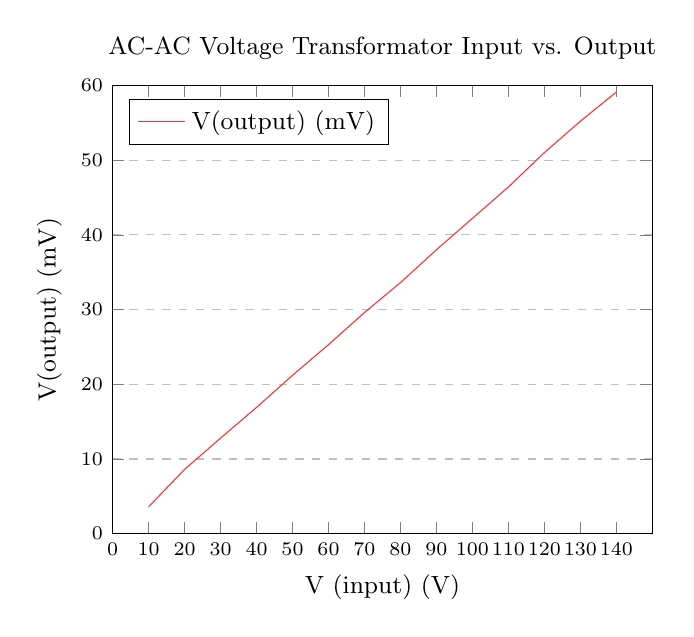
\begin{tikzpicture}
    \begin{axis}[
    title={AC-AC Voltage Transformator Input vs. Output},
    ticklabel style={font=\scriptsize},
    xlabel={V (input) (V)},
    ylabel={V(output) (mV)},
    xmin=0, xmax=150,
    ymin=0, ymax=60,
    xtick={0,10,20,30,40,50,60,70,80,90,100,110,120,130,140},
    ytick={0,10,20,30,40,50,60},
    legend pos=north west,
    ymajorgrids=true,
    grid style=dashed,
    xmajorgrids=false
]
    \addplot[
        color=red!80,
        mark=circle,
    ]
    coordinates {
        (10,3.6)(20,8.6)(30,12.8)(40,16.9)(50,21.2)(60,25.3)(70,29.6)(80,33.6)(90,38)(100,42.2)(110,46.4)(120,51)(130,55.2)(140,59.1)
    };
    \addlegendentry{V(output) (mV)}
    \label{fig:V in-out}
    \end{axis}
\end{tikzpicture}
\end{minipage}

In the plotted graph, there is a near-linear relationship between the input voltage and the output voltage, which aligns with the expected behavior of a linear voltage transformation. This data is useful for calibrating and verifying the transformer’s performance, ensuring the output voltage remains within a safe and measurable range for connected circuits, such as an Arduino
\begin{minipage}{\linewidth}
    \vspace{1cm}
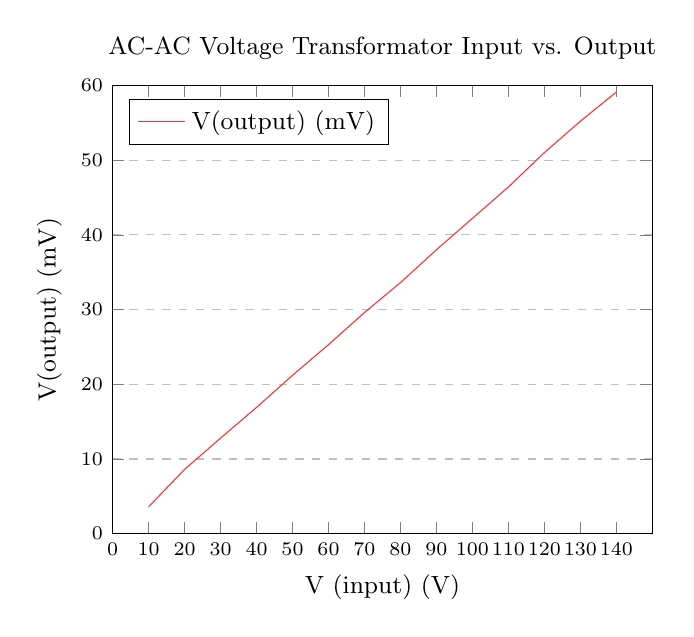
\begin{tikzpicture}
    \begin{axis}[
    title={AC-AC Voltage Transformator Input vs. Output},
    ticklabel style={font=\scriptsize},
    xlabel={V (input) (V)},
    ylabel={V(output) (mV)},
    xmin=0, xmax=150,
    ymin=0, ymax=60,
    xtick={0,10,20,30,40,50,60,70,80,90,100,110,120,130,140},
    ytick={0,10,20,30,40,50,60},
    legend pos=north west,
    ymajorgrids=true,
    grid style=dashed,
    xmajorgrids=false
]
    \addplot[
        color=red!80,
        mark=circle,
    ]
    coordinates {
        (10,3.6)(20,8.6)(30,12.8)(40,16.9)(50,21.2)(60,25.3)(70,29.6)(80,33.6)(90,38)(100,42.2)(110,46.4)(120,51)(130,55.2)(140,59.1)
    };
    \addlegendentry{V(output) (mV)}
    \label{fig:V in-out}
    \end{axis}
\end{tikzpicture}
\end{minipage}

